%% The sections on the heacy photon physics motivation.



\section{Motivations for Searching for Heavy Photons {\it Rouven}}


HPS will search for heavy photons, called $A'$s, which are new hypothesized massive vector bosons that have a small coupling 
to electrically charged matter, including electrons.  
The existence of an $A'$ is theoretically natural and could explain the discrepancy between the measured and 
observed anomalous magnetic moment of the muon and several intriguing dark matter-related anomalies.  
As discussed in the following section, HPS should also have the capability to make the first detection of \emph{true muonium}, a bound state of a 
$\mu^+ - \mu^-$ pair predicted by Quantum Electrodynamics (QED).  

The search for $A'$s has generated enormous interest in the international physics community.  This is evidenced, for example, 
by its inclusion in the recent Intensity Frontier Workshop \cite{Kamionkowski:2010mi} and by numerous  
experiments (in addition to HPS) proposed to search for them, including 
APEX~\cite{Essig:2010xa,Abrahamyan:2011gv},  MAMI~\cite{Merkel:2011ze}, and DarkLight~\cite{Freytsis:2009bh}.
We briefly review the theory and motivation for heavy photons  and then discuss updated 
reach estimates for the HPS $A'$ search.

\subsection{Theory update}

The $A'$ is a new abelian $U(1)$ gauge boson that has a weak coupling 
to electrically charged particles through ``kinetic mixing'' with the photon~\cite{Holdom:1985ag,Galison:1983pa}.  
Kinetic mixing produces an effective parity-conserving interaction
$\epsilon e A'_\mu J^\mu_{\rm EM}$ of the $A'$ to the 
electromagnetic current $J^\mu_{EM}$,  suppressed relative to the electron charge 
$e$ by the parameter $\epsilon$, which 
can naturally be in the range $10^{-12} -10^{-2}$ \cite{Essig:2009nc,Goodsell:2009xc,Cicoli:2011yh,Goodsell:2011wn}. 

An $A'$ allows ordinary matter to have a small coupling to new particles in a ``hidden sector'' 
that do not interact with the Standard Model's strong, weak, or 
electromagnetic forces.  These hidden sectors can have a rich structure and have thus far remained undetected.  
They appear in many extensions of the Standard Model, including string theory 
constructions~\cite{Goodsell:2010ie,NSF-ITP-84-170,PRINT-86-0084 (PRINCETON),Andreas:2011in,arXiv:1002.0329}
and are often required for mathematical consistency or phenomenological reasons.
The photon mixing with the $A'$ could provide the only non-gravitational window into 
their existence.   
HPS will be sensitive to $A'$ masses between 10--800~MeV. 
Such $A'$ masses can arise, for example, via the Higgs mechanism as in the models 
of~\cite{Fayet:2007ua,Cheung:2009qd,ArkaniHamed:2008qp,Morrissey:2009ur}.  

Existing constraints~\cite{endo:g2e} and the sensitivity of HPS are 
shown in Fig.~\ref{fig:hspaw-heavy-A'}. 

%%%%%%%%%%
\begin{figure*}[h]
\centering
%\vspace*{-5mm}
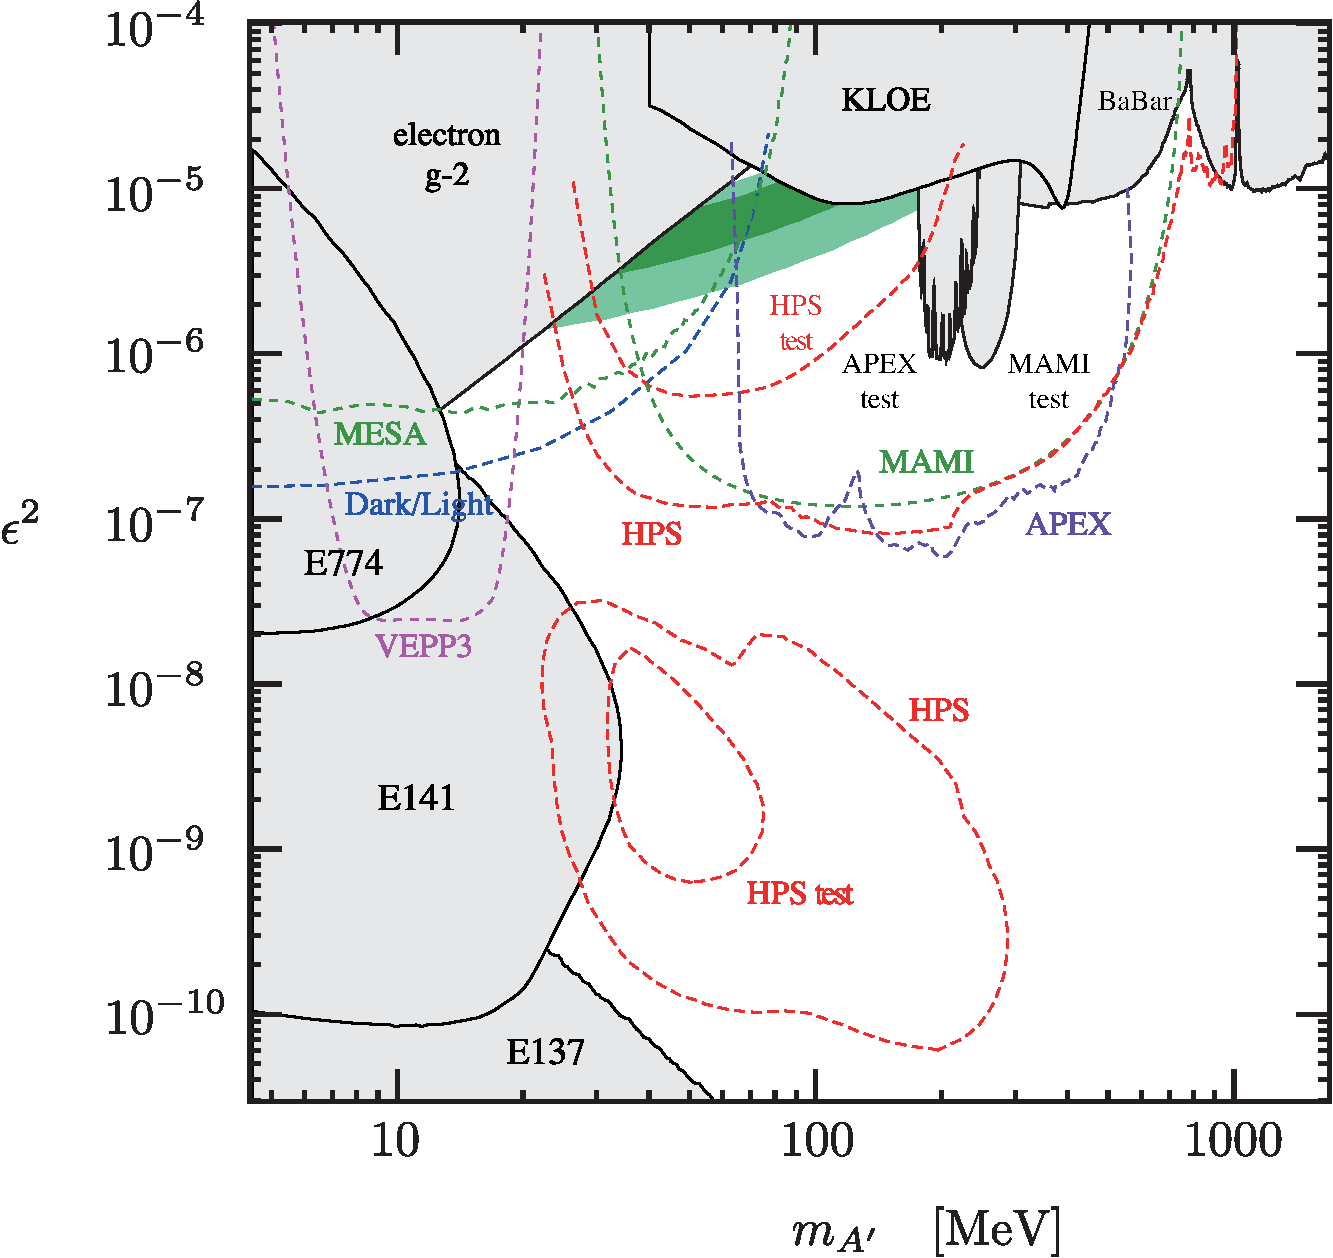
\includegraphics[width=0.7\textwidth]{limit_g-2_electron.pdf} 
\caption{
Existing constraints on heavy photons ($A'$) and the estimated HPS reach (the figure is from \cite{endo:g2e}). 
Shown are existing 90\% confidence level limits from the beam dump experiments 
E137, E141, and E774~\cite{Bjorken:2009mm,Bjorken:1988as,Riordan:1987aw,Bross:1989mp} 
the muon anomalous magnetic moment $a_\mu$~\cite{Pospelov:2008zw},  
KLOE~\cite{Collaboration:2011zc}, 
the test run results reported by APEX~\cite{Abrahamyan:2011gv} and MAMI~\cite{Merkel:2011ze}, 
an estimate using a BaBar result~\cite{Bjorken:2009mm,Reece:2009un,Aubert:2009cp},
a constraint from supernova cooling~\cite{Bjorken:2009mm} (see also~\cite{Dent:2012mx}) and a constraint from electron anomalous magnetic moment \cite{endo:g2e}.
In the green band, the $A'$ can explain the observed discrepancy between the
calculated and measured muon anomalous magnetic moment~\cite{Pospelov:2008zw} 
at 90\% confidence level.
%Projected sensitivities are shown for the full APEX run~\cite{Essig:2010xa}, 
%DarkLight~\cite{Freytsis:2009bh}, and VEPP-3~\cite{Wojtsekhowski:2009vz}.  
%MAMI has plans (not shown) to probe similar parameter regions as these experiments. 
Several projected sensitivities are shown for HPS. Solid red shows the 2$\sigma$ limits from the full HPS experiment, assuming 3 months of running time at each of 2.2 GeV(200 nA) and 6.6 GeV (450 nA). The upper region corresponds to a resonance search, the lower to a combined resonance plus vertexing search. Dashed red shows the limits from 1 week of running the HPS Test Run at 2.2 GeV (200 nA). The dashed blue limits corresponds to 1 week of running the Test Run at 1.1 GeV (200 nA).  
%Existing and future $e^+e^-$ colliders like \babar, BELLE, KLOE, Super$B$, BELLE-2, and KLOE-2  can also probe large 
%parts of the parameter space for $\epsilon\gtrsim 10^{-4}-10^{-3}$ (not shown).  
}
\label{fig:hspaw-heavy-A'}
\end{figure*}
%%%%%%%%%%


\subsubsection{Heavy Photons and Dark Matter}

The possible role of heavy photons in the physics of dark matter~\cite{ArkaniHamed:2008qn,Pospelov:2008jd} has provided an urgent impetus to search directly for heavy photons.  Results from two classes of dark matter searches --- ``indirect'' searches for galactic dark matter annihilation and ``direct'' searches for dark matter scattering off nuclei --- have both been interpreted as potential signals of dark matter interacting through a heavy photon.  Both fields have evolved in the last year, but not decisively.  New astrophysical constraints have altered the favored parameter space for dark matter annihilation into heavy photons, but a significant region remains viable, and this overlaps considerably with the projected sensitivity of HPS.  The motivation to test these theories of dark matter in a controlled laboratory experiment therefore remains strong.    Several direct-detection experiments have published conflicting bounds on dark matter scattering, and putative signals
 .  The physics of heavy-photon-mediated dark matter interaction was presented at some length in the proposal to PAC 37.  Here we briefly summarize the status of dark matter and the case for its interactions with heavy photons,  then discuss new observational constraints and theoretical developments.

The concordance model of big bang cosmology --- the Lambda Cold Dark Matter ($\Lambda$CDM) model --- explains all observations of the cosmic microwave background, large-scale structure formation, and supernovae, see 
e.g.~\cite{LambdaCDMData}. This model suggests that Standard Model particles make up only about 4\% of the energy density in the Universe, while ``dark energy'' and ``dark matter'' make up 74\% and 22\%, respectively, of the Universe's energy density. The concordance model does not require dark matter to have any new interactions beyond gravity with Standard Model particles. However, an intriguing theoretical observation, dubbed the ``WIMP miracle'', suggests that dark matter does have new interactions. In particular, if dark matter consists of ~10 GeV to 10 TeV particles interacting via an electroweak-strength force (weakly interacting massive particles or WIMPs), they would automatically have the right relic abundance consistent with the $\Lambda$CDM model.

If dark matter does interact with ordinary matter, it can interact in at least two ways: dark matter particles in the Milky Way Galaxy (and other bound astrophysical systems) can annihilate into visible matter, which could be detectable as energetic cosmic rays and/or gamma rays at Earth (indirect detection).  Dark matter passing through Earth can also scatter off nuclear targets, causing the target to recoil.  This recoil is observable in radio-pure detectors with sufficiently low background rates of nuclear recoil (direct detection).  

The satellites PAMELA \cite{Adriani:2008zr} and Fermi \cite{Ackermann:2010ij}, the balloon-borne detector ATIC \cite{Chang:2008aa}, the ground-based Cherenkov telescope HESS \cite{Aharonian:2008aa,Aharonian:2009ah}, and other experiments have all reported an excess in the cosmic-ray flux of electrons and/or positrons above backgrounds expected from normal astrophysical processes.  The evidence for this excess has only grown, with new measurements of the cosmic-ray electron flux by PAMELA \cite{Adriani:2011xv} and confirmation by Fermi of the positron excess \cite{FermiLAT:2011ab}.  It is expected that results from AMS-II will eventually shed more light on the spectrum of these excess cosmic-rays.  However, the origin of these excess positrons and electrons remains unknown.  It may plausibly arise from any of three possibilities: pair creation in nearby pulsars, acceleration in supernova shocks, or dark matter annihilation or decay.

If the excess arises from dark matter annihilation, two features are incompatible with annihilation of ``conventional'' thermal WIMP dark matter charged under the Standard Model weak interactions, but compatible with an alternative explanation, namely that dark matter is charged under a new $U(1)'$ and annihilates into $A'$ pairs, which decay directly into electrons and positrons, and/or into muons that decay into electrons and positrons (see e.g. \cite{ArkaniHamed:2008qn,Pospelov:2008jd,Cirelli:2008pk,Cholis:2008qq,Cholis:2008wq}): 
\begin{itemize}
\item The annihilation cross-section required to explain the electron signal is $50-1000$ times larger than the cross-section favored for the ``WIMP miracle''.   This can be explained if dark matter interacts with an $\mathcal{O}$(GeV)-mass $A'$, which mediates a new moderate range force and enhances the annihilation rate at low velocities (the relative velocity of dark matter in the Galactic Halo, $v\sim 10^{-3} c$, is much lower than in the early universe, and the relative velocity in self-bound dark matter subhalos is lower still).  We refer the reader to \cite{Finkbeiner:2010sm,Slatyer:2011kg} for a recent discussion.
\item The PAMELA satellite did not see any anti-proton excess \cite{Adriani:2008zq}, which implies that, if dark matter annihilation is responsible for the positron/electron signals, it does not produce baryons.  This contradicts expectations for dark matter annihilating through Standard Model interactions, but is expected if dark matter decays into light $A'$, which (for $m_{A'}\lesssim$ GeV) are kinematically unable to decay into protons and anti-protons.
\end{itemize}

Important constraints on the dark matter interpretation of these excesses arise from dark matter annihilation in other astrophysical systems (including dwarf galaxies \cite{Ackermann:2011wa}, the outer Milky Way \cite{DiffuseGalactic}, Galactic Center (e.g. \cite{Papucci:2009gd,Hutsi:2010ai} and references therein), and distant galaxies \cite{Hutsi:2010ai,extragalactic} and clusters \cite{Huang:2011xr}), and in the epoch of atomic recombination in the early universe, which leaves an imprint in the cosmic microwave background radiation \cite{CMBrefs}. 
Unfortunately, the most sensitive of the astrophysical constraints are also quite dependent on numerous astrophysical uncertainties, including the gamma-ray background fluxes and the phase-space distribution of dark matter.  

The status of models with light mediators ($\lesssim 200$ MeV), the target region for HPS, is particularly difficult to assess, because small, self-bound ``subhalos'' of dark matter with low velocity dispersions can easily enhance annihilation signals, both locally and in other galaxies.  The enhancement from subhalos in distant galaxies strengthens constraints on $A'$ models.  On the other hand, local enhancement lowers the couplings needed to explain the Fermi and PAMELA excesses, and these lower couplings are in turn less constrained by other systems.  Many analyses neglect the possibility of local subhalos, thereby overstating their exclusions of light $A'$ models.

Fits to N-body simulations do appear to favor a significant local substructure component \cite{Pieri:2009je,Kistler:2009xf,Kamionkowski:2010mi} which, in light $A'$ models, would easily dominate the local cosmic-ray signal.
	

Accounting for substructure at the level suggested by e.g.~\cite{Kamionkowski:2010mi},  light-$A'$ regions easily avoid constraints from the CMB, galactic center, dwarf galaxies, and dark matter self-interaction (though improved measurements of the CMB by Planck could severely constrain even these scenarios)~\cite{Slatyer:2011kg}.   Constraints on dark matter annihilation in distant galaxies (which would give rise to a diffuse and isotropic gamma-ray signal over the entire sky) are potentially severe even for these light-$A'$ models, but subject to theoretical uncertainties of several orders of magnitude.  In summary, light-$A'$ models of dark matter annihilation are consistent with all other data, but their viability depends on aspects of the dark matter distribution that are not yet reliably understood.

 

The search for dark-matter-nuclear scattering has also seen considerable developments recently, but remains equally ambiguous.  Three experiments have reported excesses that \emph{may} be attributable to dark matter: DAMA/Libra \cite{Bernabei:2010mq}; CoGeNT \cite{Aalseth:2010vx}, which also reported an annual modulation signal \cite{Aalseth:2011wp}, and CRESST \cite{Angloher:2011uu}.   While these experiments' signals are most readily attributed to light dark matter ($\sim 10$ GeV), results from CDMS \cite{CDMS}, XENON10 \cite{Angle:2011th}, and XENON 100 \cite{Aprile:2011hi} appear to exclude the same parameter regions.  Some model parameter space remains moderately consistent with all of these results \cite{Kelso:2011gd}.  Though the evidence for light dark matter is spotty, it does raise a puzzle: dark matter with such low masses and high couplings cannot easily interact through Standard Model forces (such as $Z$ exchange), without being excluded by measurements of the total $Z$ width at LEP. If indeed dark matter is light, then it seems most likely to interact through a new mediator, a possibility that HPS will probe.

\subsubsection{Heavy Photons and Muon $g-2$}

Besides being theoretically natural and having a possible connection to dark matter, an $A'$ could explain the discrepancy between the measured and 
calculated value of the anomalous magnetic moment of the muon $(a_\mu=g-2)$~\cite{Pospelov:2008zw}.  
This long-standing puzzle has several possible resolutions, but among the simplest new physics explanations
is the existence of a new force mediator that couples to muons, like the $A'$.  The contribution to $a_\mu$ of the $A'$ 
is like that of the photon, but suppressed by the mixing parameter $\epsilon^2$ and dependent on the $A'$ mass.  
The green region in Fig.~\ref{fig:hspaw-heavy-A'} is the 2$\sigma$ band in which the $A'$ can 
explain the discrepancy.  This is an intriguing region, which the HPS experiment will probe.  

\subsubsection{HPS physics with True Muonium}

Positronium and muonium, bound states of $(e^+ e^-)$ and $(\mu^+ e^-)$ pairs, respectively, have been
produced and studied \cite{Deutsch:1951zza,Friedman:1957mz,Hughes:1960zz}, but true muonium has not yet been 
detected (see e.g. \cite{Holvik:1986ty,ArteagaRomero:2000yh,Brodsky:2009gx,Bilenky:1969zd,Hughes:1971,Malenfant:1987tm,Karshenboim:1998we,Owen:1972,Jentschura:1997ma,Jentschura:1997tv,Karshenboim:1998am}. 
Together with tauonium $(\tau^+ \tau^-)$ and tau-muonium $(\tau^{\pm} \mu^{\mp})$, true muonium is among the most
compact pure QED systems. While $(\tau^+ \tau^-)$ and $(\tau^{\pm} \mu^{\mp})$ are difficult to detect since the $\tau$ has a
weak decay that competes with the QED decay, the $\mu$ is very long lived so that the decay of true
muonium is purely a QED process. 

The detection of true muonium would be a significant discovery and would constitute a further important test of QED.   
A number of applications of true muonium measurements have been highlighted in 
\cite{Brodsky:2009gx}, designed to exploit true muonium as a perturbative laboratory 
for QCD bound state physics. 
These include measuring dissociation cross-sections as a function of energy and lifetimes of the various states. 
More speculatively, the discrepancy between theory and experiment for $g-2$ of the muon~\cite{Bennett:2006fi} and the discrepant measurement of
the charge radius of the proton using muon bound states~\cite{Pohl:2010zza} suggest that further measurements of 
muon properties would be useful to resolve these puzzles. 


\subsection{Update on experimental status}

Some of new stuff on A$^\prime$ \cite{andreas,endo:g2e,rarek}.

% References



